\documentclass[a4page]{article}
\usepackage{fullpage}
\usepackage{url}
\usepackage[]{acronym}
\usepackage{graphicx}
\usepackage{afterpage}
\usepackage[top=1.5in, bottom=1.5in, left=1.5in, right=1.5in]{geometry}
%\usepackage{apacite}

\author{J\"org Amelunxen \\
(650 44 65)
}
\title{Master thesis proposal 
}
\date{\today}

\begin{document}
\maketitle

\newcommand{\stab}[1]{\hspace{.05\textwidth}\rlap{#1}}
\newcommand{\tab}[1]{\hspace{.1\textwidth}\rlap{#1}}

\begin{table}[!th]
\begin{tabular}{l p{0.8\textwidth}}
Supervisor & Dr. Simon Oberth\"ur \\
Project Title &  HiP - Developing a web-backend of the AR-application 'History in Paderborn' using an agile software development approach
\end{tabular}
\end{table}

\begin{abstract}
This proposal will show the planned development of the application called 'History in Paderborn'. After the application has been motivated, the proposal will include general ideas, features and background information of the system, like used respectively proposed methods and frameworks. Furthermore, the general milestones and the structure of the final thesis will be shown within the proposal. 
\end{abstract}

\section{Introduction - Current Situation}
At the present point in time, guests of the city Paderborn has to look up information about the city in a tedious way, for example using Wikipedia or other existing platforms. On the other hand, people, who want to provide information about the city (e.g., university employees or students), have to provide these information in a general accessible way, again like Wikipedia. Thus, they are limited to the features that are provided by these platforms. Since Wikipedia has been founded in 2004 by the Wikimedia foundation \cite{wikimedia}, most of the used technologies of the web application are nowadays outdated and very general. So, there is a rising need for a new technological updated approach, which is more focused on the specific topic of the city Paderborn and its history. 

Especially the use of mobile devices has been risen in this time, which is easily recognizable at the number of sales of the Apple iPhone. The iPhone has been sold 0.27 million times in Q3 2007 and 51.03 million times in Q1 2014 \cite{statIPhone}. Of course, this shift from the device side (i.e., hardware) includes a major shift in (software-) technology as well. Technologies like the nowadays well known \ac{AR} would not be possible in 2004. Of course, this new technology includes a lot of new opportunities to transfer knowledge between people and cultures. \ac{AR} is a great example to show how 'the real world' is blended more and more with artificial information; for example in the form of call-outs and layers. \ac{AR} is a technology that displays virtual (i.e., digital) information on top of a real object or location using the camera of a mobile device as input for the real objects. So, it ends up to be a combination of both worlds; the real and the digital one. Azuma et. al. has shown a lot of possible fields where the usage of \ac{AR} would be a great improvement, which includes the field of annotation and visualization \cite{Azu97}. Furthermore, path finding and navigation are fields that could be revolutionized by using \ac{AR} on mobile devices.

With a simple information website or app like Wikipedia, we include the tedious situation that the person that wants to get to the place he just read about, needs to input the address into another app to navigate him to the position. After he have arrived, he need to switch back to, for example, Wikipedia to manual compare the written information with the object or place he sees in front of him. If the person wants to change the shown information on his mobile device, he does this in general by using the touchscreen of the device. Nevertheless, he is comparing and looking at something that is placed in front of him. This leads to a break within the action and perception space \cite{ham01} and is a bad example with respect to the locality of the information \cite{Bon10}. As we will see, \ac{AR} is a tool that we can use to remove this problem and join the action and perception space while keeping the locality of the information in mind.  Furthermore, at the moment we have a lot of unnecessary overhead due to the needed app switching between the information app and the navigation app.   

Now, even if somebody wants to publish information about Paderborn on Wikipedia to enable guests of the city to get knowledge about the environment, it is only possible to publish the information as static content (that includes text, graphics, audio and video). On top of that, it is not possible to review the information privately and in enough detail to create university courses that do not include a written paper as the final exam but an entry within such an information system.  So, if we would have private annotations within a system that is owned by the university, it would enable the university employees to offer courses that fill the database about Paderborn with high quality content by students.

This leads us to the application that should be prototypical developed within this master thesis, which will be described in the next section. 
  
\section{Problem Definition - Goal of the Master Thesis} 
\label{ProblemDef}
To handle all these problems that have been described above within the section about the current situation, we will focus on the backend system for the smartphone application. The master thesis will handle the planning respectively cost estimation of the different parts/features of the system and will, after the needed technologies/frameworks are elaborated and evaluated, include a prototypical implementation of the needed components. The system should be able to get data from university courses to enable the rendering of \ac{AR} information and navigation right within the smartphone application. In the following, we will explain the two parts separately.

\subsection{The frontend: Smartphone application} 
\begin{figure}[th]
\centerline{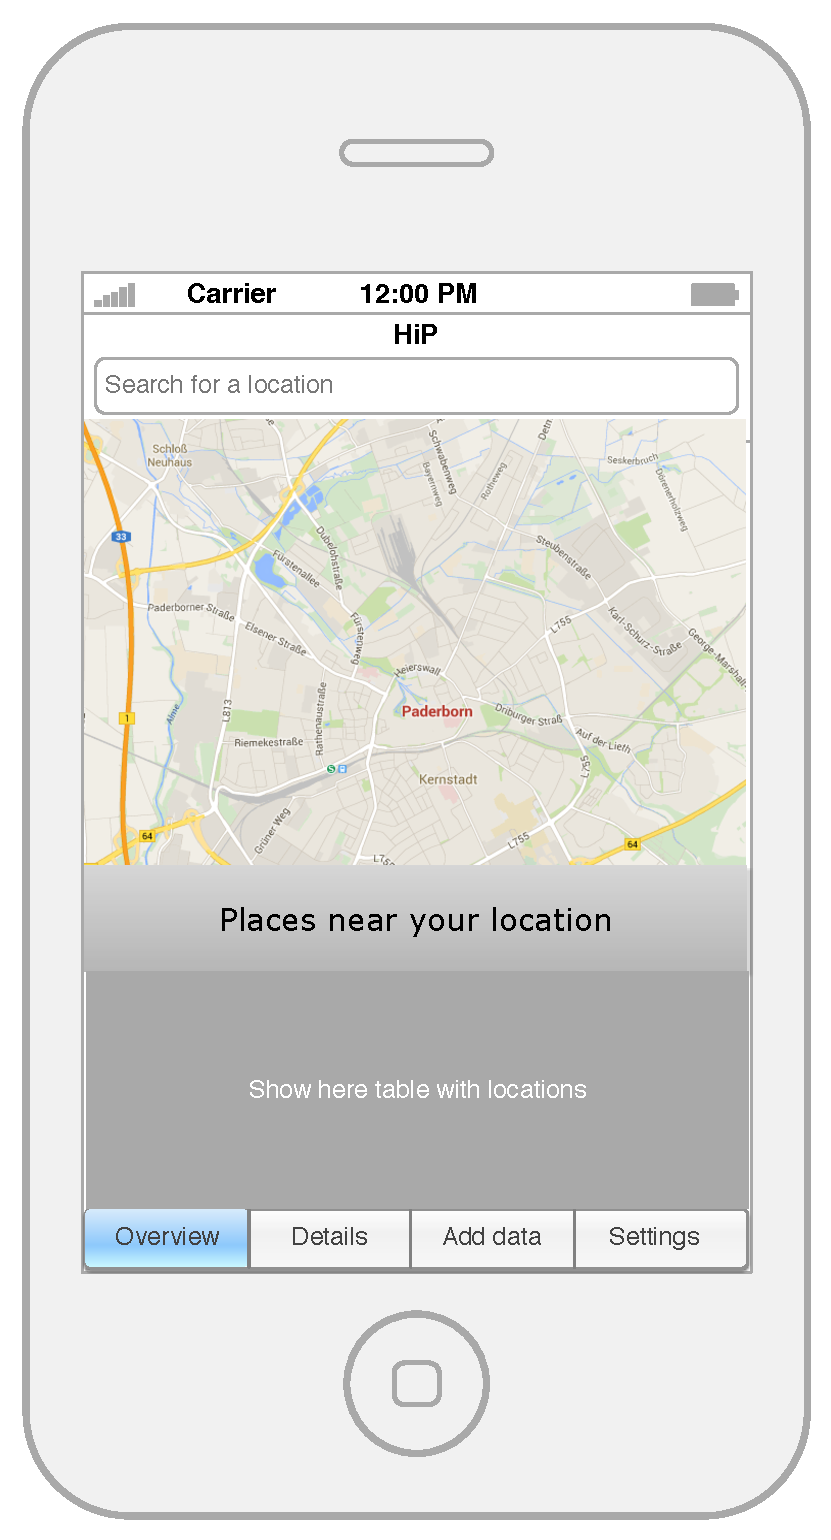
\includegraphics[width=0.5\textwidth]{gfx/mockup_app_1}}
\caption{A mockup showing the main page of the frontend application showing a map of paderborn and a general overview about the UI-elements}
\label{app1}
\end{figure}

The smartphone application is the part of the system that gets shipped to the end-user (respectively downloaded via an App-Store like Google-Play). The user can use the app to find interesting places respectively objects in Paderborn and is able to start a navigation to the place/object easily. Furthermore, the user can get an overview about all places in Paderborn by activating a map that shows all entries within the system. A mockup of this view is shown in Figure \ref{app1}. Of course, the user will be able to set up specific filters like 'show only art', 'show only historic buildings' or 'use simplified language' to adapt the system to his own experiences and educational qualifications. Moreover, if the university courses would add information over years, the system will need filtering features like this to handle the complexity of the data.

After an user has reached an interesting place, he can use the details tab to switch into the \ac{AR}-mode. With this view, the user can use the smartphone-camera to embed information, which has been added via the backend, right into the picture of the object. An mockup of this view is shown in Figure \ref{app2}. 
To create a feasible input for the \ac{AR} system, the user should be able to scan objects in 3D right with his smartphone application and send the data (i.e., a point-cloud of the scanned object), back to the web-server.  Afterwards, the user can add annotations to the point-cloud via the web-backend of the system.  

\begin{figure}[th]
\centerline{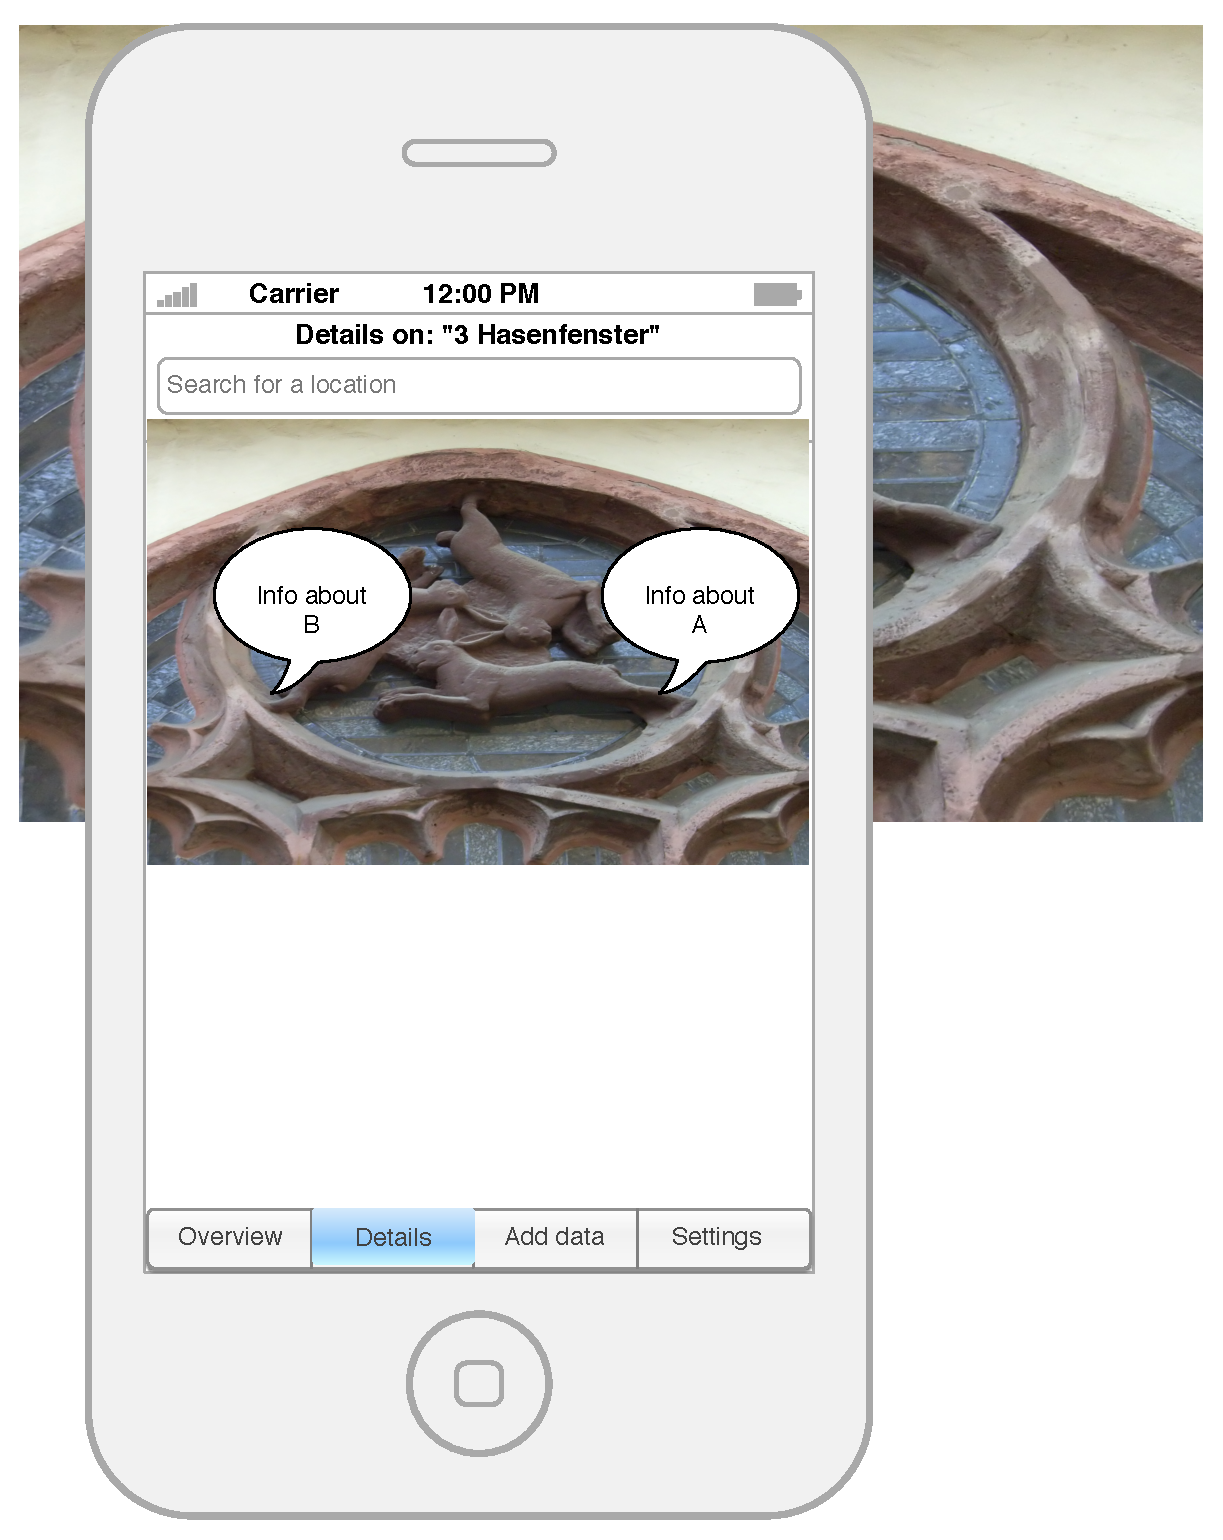
\includegraphics[width=0.7\textwidth]{gfx/mockup_app_2}}
\caption{A mockup showing the details page of the "Dreihasenfenster" while the camera of the smartphone is pointing to the window itself}
\label{app2}
\end{figure}

\subsection{The backend: Web-Server} 
Another important part of the system, and the main focus of the master thesis, is contained within the backend-web-server. The backend should contain the whole data handling and assessment. The students should be able to add data to the system (e.g., a textual article, graphics, \ac{AR}-data, etc.) and to modify existing data via a \ac{CMS}. These entries get reviewed, for example by the course supervisor, and unlocked for the frontend application. To do this, the backend needs features like annotations and highlighting, which should be private for a specific user. By using this, the supervisor can evaluate the given texts right within the \ac{CMS} and give his final judgement. If the supervisor is not satisfied with the quality of the given text, he should be able to send the document back to the student, to get a revised and updated version of the document. If the supervisor is satisfied, he can unlock the information for showing in the frontend application.

The data should be stored in a way that it can be shown within an \ac{AR}-environment in the smartphone application. Of course, we will need some mechanism to structure the data, for example tags or stored categories. This kind of information (especially tags) are also very important for the described filtering techniques on the client side.

\begin{figure}[th]
\centerline{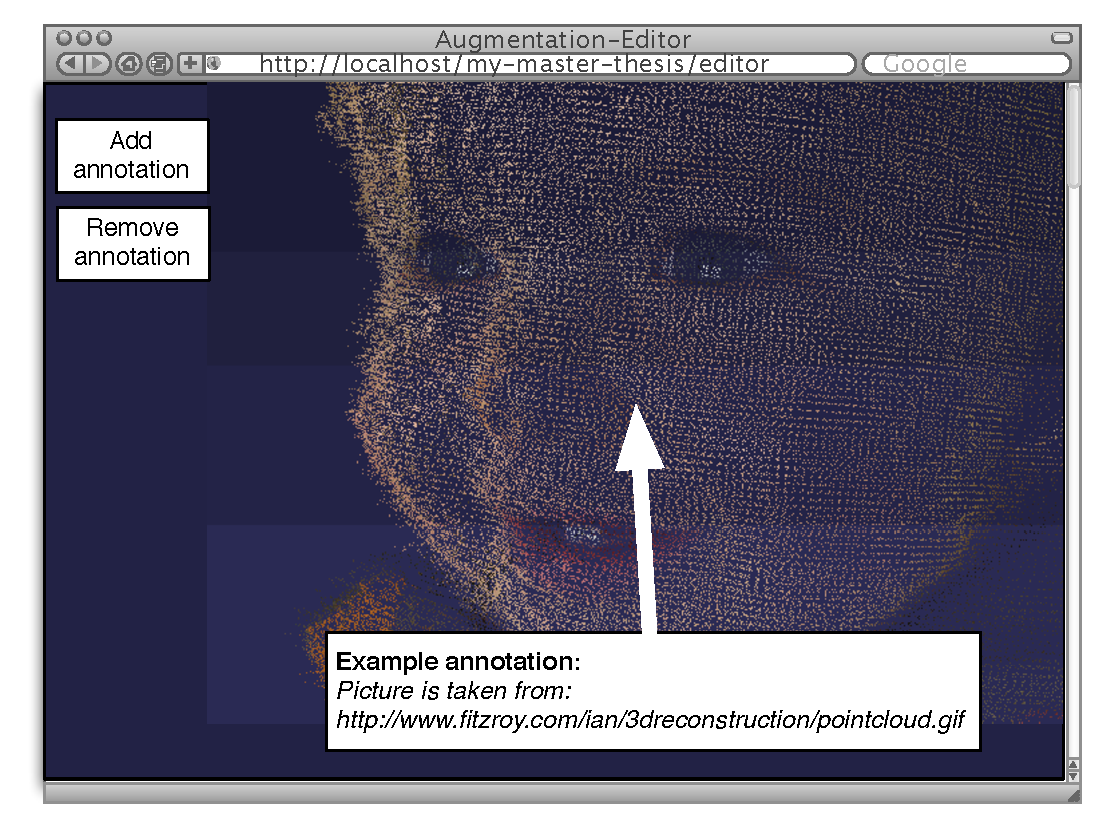
\includegraphics[width=1\textwidth]{gfx/mockup_web_1}}
\caption{A mockup showing the augmentation editor that will be included in the web-application. The editor will be used to edit the point-clouds, which have been added with the help of the smartphone-application}
\label{web1}
\end{figure}

Furthermore, the backend should include a way to modify the point-clouds of the objects that has been scanned with the smartphone application. It will need features to add annotations directly to these point-clouds to show them afterwards within the \ac{AR}-environment. This editor will be created on the basis of \ac{HTML5} and \ac{WebGL}. A mockup of this site is shown in Figure \ref{web1}. These annotations should also be assessable and (un-)lockable for the supervisor. 

\subsection{The system as a whole}
So, as we have seen in the two sections about the server and the client side, we will have mainly three different user groups, who interact with the system. One group includes the students, who want to add information to the database via the backend-\ac{CMS} to get a mark. Another user group consists of the supervisors of the university courses. They should be able to review the data that has been included via the students and (un-)lock the data for the frontend. The last group contains the users of the system, who do not want to add information but use the app for information and navigation purposes within Paderborn. These users do not have any rights to change things but can use the information pages, the \ac{AR}-view of the app and the navigation features. 

If a user requests an \ac{AR}-object within the app, the point-cloud will be loaded from the web-server. After that, the smartphone app will show the annotations within an \ac{AR}-environment by synchronizing the corresponding point cloud to the object that is currently focused with the internal camera of the smartphone. This process is also shown in Figure \ref{sdia1} as a high level \ac{UML}-sequence diagram.

\begin{figure}[th]
\centerline{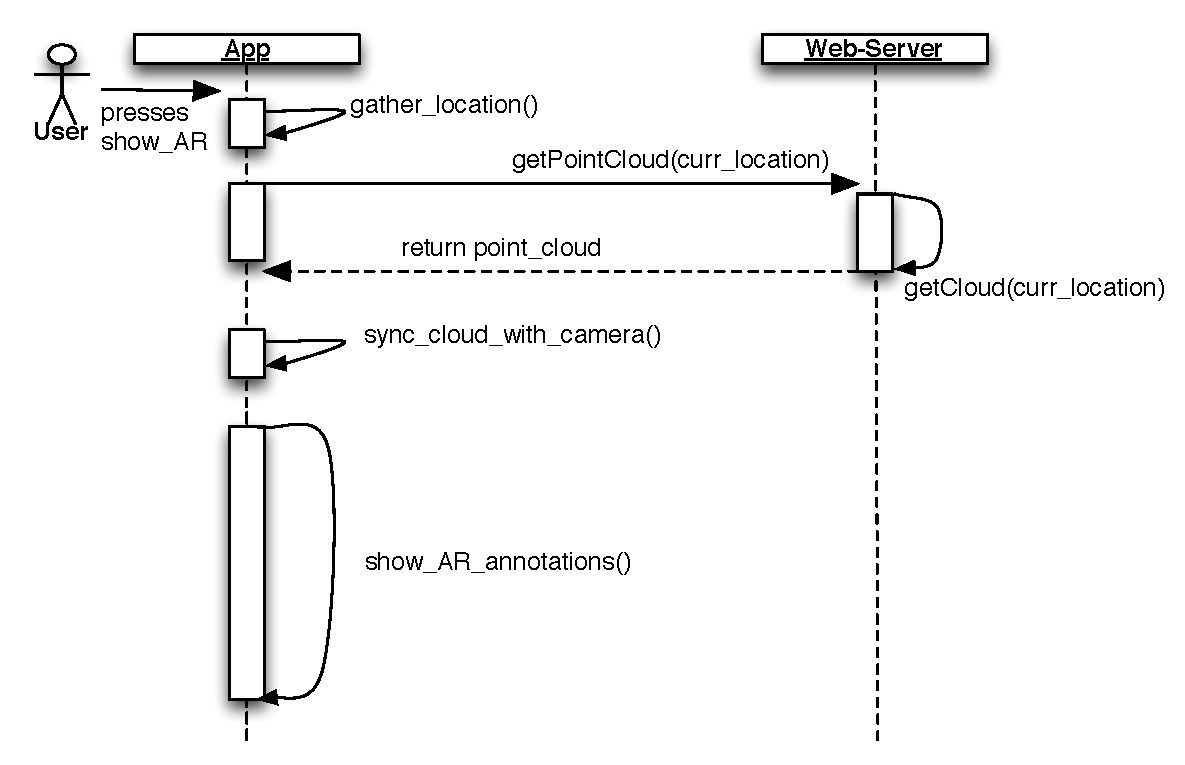
\includegraphics[width=1\textwidth]{gfx/sdia1}}
\caption{A simple sequence diagram showing the communication between the server and the client if a user wants to enter the \ac{AR}-mode for a specific object}
\label{sdia1}
\end{figure}

Now, after we have seen the application that should be developed within this master thesis, we will take a look at the needed methods and frameworks that will be needed within the thesis to create the system within the given timeframe. 

\section{(Methological-)background of the thesis}
This section will contain information about the needed frameworks and methods to create an application like the one that has been described in section \ref{ProblemDef}.
\subsection{Used frameworks}
We will need a couple of frameworks and libraries to create such a big project in the existing timeframe. These frameworks will handle mainly two big parts of the system; on the one hand the \ac{AR}-scanning of the objects and presentation and, on the other hand, we will use the Play-framework to speed up the development process of the web-server backend. But, at first we will describe the \ac{AR}-frameworks.

\subsubsection{AR frameworks}
A possible framework to use within the \ac{AR}-context is Wikitude. It runs on Android and iOS an handles the image recognition, image tracking, 3D model rendering and video overlay \cite{wikitude}. Thus, the Wikitude framework would be a great help within the development of the frontend. The framework is not open source but it is free for educational projects (including a forced starting animation and Wikitude logo in camera view).  

Another possible basis is the usage of the augmented reality browser Junaio. The company Metaio, which runs Junaio, offers a developer program to develop own applications on the basis of the Junaio (eco-)system. Moreover, it is completely free of charge for the developers \cite{junaio1}. However, deployed apps will be shipped with a Metaio watermark inside as long as you do not buy a specific license. 

Another important aspect is a framework that handles the backend. Such a framework is the Play-framework, which will be described in the following.
\subsubsection{Play}
The Play-framework is an open source web application framework that can be used to create web applications that rely on the \ac{REST} principle. \acf{REST} is a general style of software architecture that is used to build distributed systems and has been introduced in the dissertation of \cite{Fielding2000}. 
As Rodriguez et. al. point out, \ac{REST} based web services are easier to use than \acf{SOAP} and \acf{WSDL}-based ones and getting more and more importance since mainstream web 2.0 service providers are taking up on \ac{REST}\cite{Rodriguez2008}. Furthermore, the Play-framework comes with integrated unit testing and full support of asynchronous I/O. So, all in all, Play will noticeably enhance the development speed of the backend.

After we have seen a couple of frameworks, which will needed within the master thesis, we will now take a look at methods that will also play a major role within the development process.

\subsection{Used methods}
\label{SCRUM}
Since the application should be able to handle the input of first datasets within the summer semester 2015, we will need a fast development process, which is closely coupled to the needs of the customer - in our case the humanities scholars of the university of Paderborn. 

Because of that, the application will be development with a SCRUM development process. This means, the application will be developed within autonomous short 'sprints' with a length between 1 up to 4 weeks. After every sprint the product should be more refined \cite{scrum}. However, it should be possible to execute the application at the end of any given sprint, which will result in a fast and stable development process. Moreover, SCRUM is known to reduce every category of work (i.e., defects, rework, total work required, and process overhead) within a \ac{CMMI} compliant development process by almost 50\% \cite{Sut09}, which is also great for development in this short timeframe.
The development process also influences the order of the development because the chose of SCRUM indicates that we will develop the front-end and back-end in parallel. We will use a \ac{TDD}-like approach within every sprint (where possible). So, we will at first create needed test cases and afterwards implement against these test cases. This approach will prevent that testing of the application will be shifted into the last week(s) of the development process and done in a superficial way. In addition to that, a comprehensive test suite is a great basis for further development \cite{max03}.

Furthermore, since we will need to specify the possibilities within this timeframe of 20 weeks, we will need methods for cost estimation to get an idea about the general complexity and, thus, the needed time to finish the features. If we find useful features, that are not create-able in this short period of time, then these features will be included and described in the future work section of the final thesis. A possible method for this estimation is the \textit{Analysis effort method}. However, since we will use SCRUM, an estimation is also possible by summing up the expected work for every planned feature within a specific sprint (respectively for the whole project).

At this point, we have finished the theoretical part of the thesis description. Now, we will take a closer look at the planned general structure of the thesis.

\section{General structure of the thesis}
The thesis will include a general part that contains the needed background information to understand the following development. Furthermore, this part will evaluate a couple of frameworks that will be used within the development process and describe why these frameworks are used in the first place. Another important part of the section will be the description of SCRUM that will be used as a development method.  

After that the thesis will describe the implementation details and offer insights into the testing procedure (on the technical and user side) and will draw a general conclusion about the whole project and will include a look into the future with respect to possible future work. Note that, of course, this structure is not fixed and may be changed a little bit in the future. \\

\begin{tabular}[th]{lll} 
Content of the thesis:  		& 	1 Introduction									&  \\ 
 			& \stab{1.1 What is the current situation without the tool/app} 	&  \\
 			& \stab{1.2 What would the system look like (briefly)	}		&  \\
 			& \stab{1.3 What would be better if the app would exit? Who would benefit?} 		&  \\
   			& 2 Technical and methodological background			&  \\ 				 	
  			& \stab{2.1 Agile Development - Scrum}					&  \\ 
			& \stab{2.2 Methods for cost estimation}					& \\
  			& \stab{2.3 Used Frameworks}							&  \\ 
  			& \tab{2.3.1 Play Framework Backend}					&  \\ 
  			& \stab{2.4 WebGL}									&  \\ 
 			& \stab{2.5 Tooling}									&  \\ 
 			& \tab{2.5.1 Git} 									&  \\ 
			& \tab{2.5.2 Jira}									&  \\ 
 			& \tab{2.5.3 Eclipse - Plugins -}							&  \\ 
  			& \stab{2.6 Testing techniques}						&  \\ 
  			& \tab{2.6.1 Why is testing within an agile development even more important}&  \\ 
  			& \tab{2.6.2 TDD}									&  \\ 
  			& \tab{2.6.3 The fundamental test process}				&  \\ 
  			& 3 Draft of the	application							&  \\ 
  			& \stab{3.1 Backend (Web-Server)}						&  \\ 
			& \tab{3.1.1 Cost estimation of the backend}				& \\
  			& \tab{3.1.2 Input data/content via CMS in the system}		&  \\ 
  			& \tab{3.1.3 Manage content as a reviewer}				&  \\ 
  			& \tab{3.1.4  Including a 3D-Tooling system for point-clouds (WebGL)}&  \\ 
  			& \stab{3.2 Frontend (App)}							&  \\ 
			& \tab{3.1.1 Cost estimation of the frontend}				& \\
  			& \tab{3.2.2 Input data into the system (scan objects and annotate them)} &  \\ 
  			& \tab{3.2.3 Show close "interesting places" within a map /  via a overlay} &  \\ 
  			& \tab{3.2.4 Navigation to "interesting places"}				&  \\ 
  			& \stab{3.3 Interface}							&  \\ 
			& \tab{3.3.1 Data format for \ac{AR} files}				& \\
  			& 4 Implementation details							&  \\   							& 5 Testing results									&  \\ 
  			& 6 Acceptance test of the prototype						&  \\ 
  			& \stab{6.1 Small usablity study of the app}				&  \\ 
  			& \stab{6.2 Small usability study of the backend / CMS}		&  \\ 
  			& 7 Conclusion 									&  \\ 
  			& \stab{7.1 Results}									&  \\ 
  			& \stab{7.2 Future Work / What can be improved?}			&  \\ 
\end{tabular} \\

Now, after we have seen the planned general structure of the thesis, we will come to the planned timing.
\clearpage
\section{Time Managment and milestones}
\begin{figure}[h]
\centerline{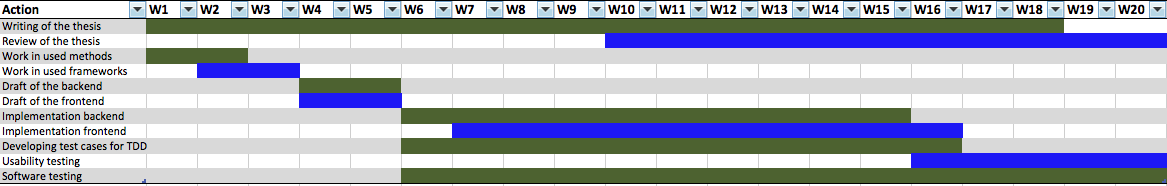
\includegraphics[angle=90,origin=c,width=0.23\textwidth]{gfx/gantt_ss}}
\caption{The expected timing shown as a Gantt diagram}
\label{gantt}
\thispagestyle{empty}
\end{figure}

\begin{table}[h]
\centering% NICHT \begin{center}
\begin{tabular}{lll}
Week  		& 	Action				&  \\
\hline 
 1-18		&Writing of the thesis		&  \\
 10-20		& Review of the thesis		&  \\
 1-3			& Work in used methods		&  \\
  2-4 			& Work in used frameworks	&  \\ 				 	
  4-6			& Draft of the backend		&  \\ 
  4-6			& Draft of the frontend		& \\
  6-16		& Implementation backend	&  \\ 
  7-18		& Implementation frontend	&  \\ 
  6-18		& Developing Test Cases for TDD	&  \\ 
 16-20		& Usability testing				&  \\ 
 6-20		& Software testing				&  \\ 
\hline
\end{tabular}
\caption{Showing the expected timing of the thesis within a table}
\label{tgantt}
\end{table}

The expected timing is shown in Table \ref{tgantt} and more visual within Figure \ref{gantt} as a Gantt diagram. The thesis will be written over the most part of the timeframe of the 20 weeks. The last weeks are planned to include in general review and (usability-)testing work to finalize the thesis. The first milestone should be reached within Week 6 and indicates the finish of the draft and the start of the actual implementation. 

The second milestone should be reached in Week 17 and indicates the end of the implementation phase. The frontend and backend will mainly be implemented in parallel because we will use SCRUM as the main development method. This means that we will have a fully working but growing systems that needs both components in the development phase to complete the SCRUM sprints, as it has been introduced in section \ref{SCRUM}. 

\section{Summary of the goals of the thesis}
The following section will now briefly summarize the goals of the master thesis:
\begin{itemize}
	\item We will need to draft the application before the actual implementation phase start, to do this, we will need:
	\begin{itemize}
	\item to collect the high level requirements %rest in den meetings
	\item to create drafts of the general architecture and the main components from these requirements
	\item to create cost estimations about the different parts of the system based on the drafts
	\end{itemize} 
	\item After that, we will implement the backend and a prototype of the frontend application %konkreter - agile zyklus -> Prozess soll durchlaufen werden
	%Welche Vorteile? Doku
	\item Finally, we will need to evaluate a suitable way to pass the whole project to an upcoming 
	'Project Group' of the AG Engels.  
	\item The whole project will be done in an agile approach using common agile project management  applications and techniques
\end{itemize} 

So, after the complete project has now been proposed and and the methods and used frameworks has been explained, we are now looking forward to create the proposed system in the following months.

\clearpage

\section*{Used acronyms}
\begin{acronym}[somethinglonger]
 \acro{AR}{Augmented Reality}
\acro{CMMI}{Capability Maturity Model Integration}
\acro{CMS}{Content-Management-System}
\acro{ECTS}{European Credit Transfer System}
\acro{HTML5}{Hypertext Markup Language 5}
\acro{HTTP}{Hypertext Transfer Protocol}
\acro{REST}{Representational state transfer}
%\acro{JSON}{JavaScript Object Notation}
\acro{SOAP}{Simple Object Access Protocol}
 \acro{TDD}{Test-Driven-Development}
\acro{UML}{Unified Modeling Language}
\acro{WebGL}{Web Graphics Library}
\acro{WSDL}{Web Services Description Language}
%\acro{XML}{Extensible Markup Language}
\end{acronym}

\bibliography{lit}
\bibliographystyle{alpha}

\end{document}


